\documentclass{beamer}
\usepackage{graphicx}
\usepackage{tikz}
\usepackage{algorithm}
\usepackage{algpseudocode}


%THEME and COLORTHEME
\usetheme{Madrid}
%\usetheme{Berkeley}
%\usetheme{Copenhagen}

%\usecolortheme{spruce}
%\usecolortheme{beetle}
%\usecolortheme{seahorse}
%\usecolortheme{wolverine}

\title{Hopcroft-Karp Algorithm}

%\subtitle{An Introduction}

\author[Rakib,Sany,Bijoy]{1905047-Rakib Abdullah\\1905048-Al-Amin Sany\\1905052-Bijoy Ahmed Saiem}

\institute[CSE, BUET]
{
Department of Computer Science and Engineering\\
Bangladesh University of Engineering and Technology
}

\date{\today}

%\logo{\includegraphics[height=1cm]{overleaf.png}}

% PLACING ToC AT THE BEGINNING OF EACH SECTION
\AtBeginSection[]
{
\begin{frame}
\frametitle{Table of Contents}
\tableofcontents[currentsection]
\end{frame}
}

\begin{document}

\frame{\titlepage}

%TABLE OF CONTENTS
\begin{frame}
\tableofcontents
\end{frame}

\section{Introduction}
\begin{frame}{Introduction}
\begin{block}{Hopcroft-Karp Algorithm}
The Hopcroft-Karp algorithm is a graph algorithm that finds the maximum cardinality matching in a bipartite graph.
\end{block} \pause
\begin{columns}[T]
\begin{column}{0.5\textwidth}
\centering
\begin{figure}
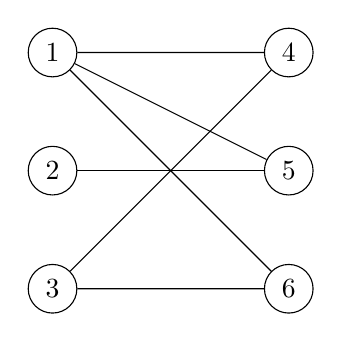
\begin{tikzpicture}[scale=1.5]
  \node[draw, circle] (a1) at (0,1) {1};
  \node[draw, circle] (a2) at (0,0) {2};
  \node[draw, circle] (a3) at (0,-1) {3};
  \node[draw, circle] (b1) at (2,1) {4};
  \node[draw, circle] (b2) at (2,0) {5};
  \node[draw, circle] (b3) at (2,-1) {6};
  
  \draw (a1) -- (b1);
  \draw (a1) -- (b2);
  \draw (a1) -- (b3);
  \draw (a2) -- (b2);
  \draw (a3) -- (b1);
  \draw (a3) -- (b3);
\end{tikzpicture}
\caption{Bipartite graph}
\end{figure}
\end{column}
\pause
\begin{column}{0.5\textwidth}
\centering
\begin{figure}
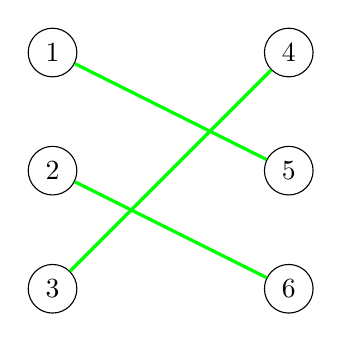
\begin{tikzpicture}[scale=1.5]
  \node[draw, circle] (a1) at (0,1) {1};
  \node[draw, circle] (a2) at (0,0) {2};
  \node[draw, circle] (a3) at (0,-1) {3};
  \node[draw, circle] (b1) at (2,1) {4};
  \node[draw, circle] (b2) at (2,0) {5};
  \node[draw, circle] (b3) at (2,-1) {6};
  
  \draw[green, very thick] (a1) -- (b2);
  \draw[green, very thick] (a2) -- (b3);
  \draw[green, very thick] (a3) -- (b1);
\end{tikzpicture}
\caption{Maximum cardinality matching}
\end{figure}
\end{column}
\end{columns}
\end{frame}

\section{Definitions}
\begin{frame}{Definitions}
     \begin{block}{Bipartite Graph}
A graph is bipartite if its vertices can be divided into two disjoint sets such that every edge connects a vertex in one set to a vertex in the other set.
\end{block}
 \pause
\begin{block}{Maximum Cardinality}
A matching in a graph is a set of edges such that no two edges share a common vertex.Maximum cardinality means maximum possible matching.
\end{block} \pause
\begin{block}{Free vertex}
 A free vertex is a vertex with no matching edge connected to it.
\end{block}


\end{frame}

\section{Algorithm}
\begin{frame}{Algorithm}
\renewcommand{\thealgorithm}{}
\begin{algorithm}[H]
\floatname{algorithm}{}
\caption{Hopcroft-Karp(G)}
\begin{algorithmic}[1]
\State $M=\phi$ \pause
\While{$P\neq\phi$} \pause
\State $P=\{p_1,p_2,\dot,p_k\}$ {\small //vertex-disjoint shortest augmenting paths} \pause
\State $M:=M\oplus\{p_1 \cup p_2 \cup \dots \cup p_k\}$\pause
\EndWhile
\State Output the matching $M$ as the maximum cardinality matching.
\end{algorithmic}
\end{algorithm}
\end{frame}

\begin{frame}{Example}
A bipartite graph is given below where we will find its maximum cardinality mathching:\\
 \vspace{.5cm}
    \centering
\begin{tikzpicture}[scale=1.5]
\tikzset{vertex/.style = {shape=circle,draw,minimum size=1.5em}}
\tikzset{edge/.style = {->,> = latex'}}

% Left partition
\node[vertex] (A) at (-2,2) {$a$};
\node[vertex] (B) at (-2,1) {$b$};
\node[vertex] (C) at (-2,0) {$c$};
\node[vertex] (D) at (-2,-1) {$d$};

% Right partition
\node[vertex] (E) at (2,2) {$e$};
\node[vertex] (F) at (2,1) {$f$};
\node[vertex] (G) at (2,0) {$g$};
\node[vertex] (H) at (2,-1) {$h$};

% Edges
\draw[edge] (A) to (E);
\draw[edge] (A) to (F);
\draw[edge] (A) to (H);
\draw[edge] (B) to (E);
\draw[edge] (C) to (F);
\draw[edge] (D) to (E);
\draw[edge] (D) to (F);
\draw[edge] (D) to (G);
\draw[edge] (D) to (H);
\end{tikzpicture}
\end{frame}

\begin{frame}{First iteration:BFS}
\only<1>{$\hspace{4.5cm}F=\{\}$}\\ % will only appear on slide 1
\only<2>{$\hspace{4.5cm}F=\{\textcolor{red}{e},\textcolor{red}{f},\textcolor{red}{h}\}$}\\ % will appear on slides 2 and later
\only<3>{$\hspace{4.5cm}F=\{e,f,h\}$}\\
\only<4>{$\hspace{4.5cm}F=\{e,f,h\}$}\\
\only<5>{$\hspace{4.5cm}F=\{e,f,h,\textcolor{red}{g}\}$}\\
\vspace{.5cm}
\hspace{2.7cm}
    \begin{tikzpicture}[scale=1.5]
\tikzset{vertex/.style = {shape=circle,draw,minimum size=1.5em}}
\tikzset{edge/.style = {->,> = latex'}}
\tikzset{red vertex/.style={vertex,fill=red!50}}
\tikzset{blue vertex/.style={vertex,fill=blue!50}}

% Left partition
\node[blue vertex] (A) at (-2,2) {$a$};
\node[blue vertex] (B) at (-2,1) {$b$};
\node[blue vertex] (C) at (-2,0) {$c$};
\node[blue vertex] (D) at (-2,-1) {$d$};

% Right partition
\node[blue vertex] (E) at (2,2) {$e$};
\node[blue vertex] (F) at (2,1) {$f$};
\node[blue vertex] (G) at (2,0) {$g$};
\node[blue vertex] (H) at (2,-1) {$h$};

% Edges
\draw[edge] (A) to (E);
\draw[edge] (A) to (F);
\draw[edge] (A) to (H);
\draw[edge] (B) to (E);
\draw[edge] (C) to (F);
\draw[edge] (D) to (E);
\draw[edge] (D) to (F);
\draw[edge] (D) to (G);
\draw[edge,color] (D) to (H);

% BFS
\onslide<2->{
%\node[blue vertex] (B) at (-2,1) {$b$};
\draw[edge,color=red] (A) to (E);
\draw[edge,color=red] (A) to (F);
\draw[edge,color=red] (A) to (H);
}

\onslide<3->{
\draw[edge,color=red] (B) to (E);
}

\onslide<4->{
\draw[edge,color=red] (C) to (F);
}

\onslide<5->{
\draw[edge,color=red] (D) to (E);
\draw[edge,color=red] (D) to (F);
\draw[edge,color=red] (D) to (G);
\draw[edge,color=red] (D) to (H);
}

\end{tikzpicture} 

\end{frame}


\begin{frame}{First iteration:DFS}
    
    \only<1-3>{$\hspace{4.6cm}F=\{\textcolor{red}{e},f,h,g\}$}\\
    \only<1-3>{$\hspace{4.6cm}P=\{(e-a)\}$}\\
    \only<4>{$\hspace{4.6cm}F=\{e,\textcolor{red}{f},h,g\}$}\\
    \only<4>{$\hspace{4.6cm}P=\{(e-a),(c-f)\}$}\\
    \only<5>{$\hspace{4.6cm}F=\{e,f,h,g\}$}\\
    \only<5>{$\hspace{4.6cm}P=\{(e-a),(c-f)\}$}\\
    \only<6>{$\hspace{4.6cm}F=\{e,f,h,\textcolor{red}{g}\}$}\\
    \only<6>{$\hspace{4.6cm}P=\{(e-a),(c-f),(g-d)\}$}\\
    \only<7>{$\hspace{4.6cm}F=\{e,f,h,g\}$}\\
    \only<7>{$\hspace{4.6cm}P=\{(e-a),(c-f),(g-d)\}$}\\
\vspace{.5cm}
\hspace{2.7cm}
    \begin{tikzpicture}[scale=1.5]
\tikzset{vertex/.style = {shape=circle,draw,minimum size=1.5em}}
\tikzset{edge/.style = {->,> = latex'}}
\tikzset{red vertex/.style={vertex,fill=red!50}}
\tikzset{blue vertex/.style={vertex,fill=blue!50}}


% Left partition
\node[red vertex] (A) at (-2,2) {$a$};
\node[blue vertex] (B) at (-2,1) {$b$};
\node[blue vertex] (C) at (-2,0) {$c$};
\node[blue vertex] (D) at (-2,-1) {$d$};

% Right partition
\node[blue vertex] (E) at (2,2) {$e$};
\node[blue vertex] (F) at (2,1) {$f$};
\node[blue vertex] (G) at (2,0) {$g$};
\node[blue vertex] (H) at (2,-1) {$h$};

% Edges
\node[red vertex] (E) at (2,2) {$e$};
\draw[edge,color=green,line width=1.5pt] (A) to (E);
\draw[edge,color=red] (A) to (F);
\draw[edge,color=red] (A) to (H);
\draw[edge,color=red] (B) to (E);
\draw[edge,color=red] (C) to (F);
\draw[edge,color=red] (D) to (E);
\draw[edge,color=red] (D) to (F);
\draw[edge,color=red] (D) to (G);
\draw[edge,color=red] (D) to (H);

\pause

\draw[edge,color=white,line width=3pt] (A) to (E);

\draw[edge,color=white,line width=3pt] (A) to (F);
\draw[edge,color=white,line width=3pt] (A) to (H);
\draw[edge,color=white,line width=3pt] (B) to (E);
\draw[edge,color=red] (C) to (F);
\draw[edge,color=white,line width=1pt] (D) to (E);
\draw[edge,color=red,line width=1pt] (C) to (F);
\draw[edge,color=red,line width=1pt] (D) to (F);
\draw[edge,color=red,line width=1pt] (D) to (G);
\draw[edge,color=red,line width=1pt] (D) to (H);




\pause
\node[shape=circle,draw=white,minimum size=2em,fill=white] (A) at (-2,2) {};
\node[shape=circle,draw=white,minimum size=2em,fill=white] (A) at ((-2,1) {};
\node[shape=circle,draw=white,minimum size=2em,fill=white] (A) at (2,2) {};

\pause  
\draw[edge,color=green,line width=1.5pt] (C) to (F);
\node[red vertex] (F) at (2,1) {$f$};
\node[red vertex] (C) at (-2,0) {$c$};

\pause
\draw[edge,color=white,line width=3pt] (C) to (F);
\draw[edge,color=white,line width=3pt] (D) to (F);
\node[shape=circle,draw=white,minimum size=2em,fill=white] (A) at (-2,0) {};
\node[shape=circle,draw=white,minimum size=2em,fill=white] (A) at (2,1) {};

\pause
\draw[edge,color=green,line width=1.5pt] (D) to (G);
\node[red vertex] (G) at (2,0) {$g$};
\node[red vertex] (D) at (-2,-1) {$d$};

\pause
\draw[edge,color=white,line width=3pt] (D) to (G);
\draw[edge,color=white,line width=3pt] (D) to (H);
\node[shape=circle,draw=white,minimum size=2em,fill=white] (A) at (2,0) {};
\node[shape=circle,draw=white,minimum size=2em,fill=white] (A) at (-2,-1) 


\end{tikzpicture}
\end{frame}

\begin{frame}{After first iteration}
After running the DFS on the remaining part, $$M=\{e-a,f-c,g-d\}$$ \\
\vspace{.35cm}
\hspace{2.7cm}
    \begin{tikzpicture}[scale=1.5]
\tikzset{vertex/.style = {shape=circle,draw,minimum size=1.5em}}
\tikzset{edge/.style = {->,> = latex'}}
\tikzset{red vertex/.style={vertex,fill=red!50}}
\tikzset{blue vertex/.style={vertex,fill=blue!50}}

% Left partition
\node[red vertex] (A) at (-2,2) {$a$};
\node[blue vertex] (B) at (-2,1) {$b$};
\node[red vertex] (C) at (-2,0) {$c$};
\node[red vertex] (D) at (-2,-1) {$d$};

% Right partition
\node[red vertex] (E) at (2,2) {$e$};
\node[red vertex] (F) at (2,1) {$f$};
\node[red vertex] (G) at (2,0) {$g$};
\node[blue vertex] (H) at (2,-1) {$h$};

% Edges
\draw[edge,color=green,line width=1.5pt] (A) to (E);
\draw[edge] (A) to (F);
\draw[edge] (A) to (H);
\draw[edge] (B) to (E);
\draw[edge,color=green,line width=1.5pt] (C) to (F);
\draw[edge] (D) to (E);
\draw[edge] (D) to (F);
\draw[edge,color=green,line width=1.5pt] (D) to (G);
\draw[edge,color] (D) to (H);
\end{tikzpicture}
\end{frame}

\begin{frame}{Second iteration}
    Running BFS on the free vertices of left side..\\
    \vspace{.5cm}
\hspace{2.7cm}
    \begin{tikzpicture}[scale=1.5]
\tikzset{vertex/.style = {shape=circle,draw,minimum size=1.5em}}
\tikzset{edge/.style = {->,> = latex'}}
\tikzset{red vertex/.style={vertex,fill=red!50}}
\tikzset{blue vertex/.style={vertex,fill=blue!50}}

% Left partition
\node[red vertex] (A) at (-2,2) {$a$};
\node[blue vertex] (B) at (-2,1) {$b$};
\node[red vertex] (C) at (-2,0) {$c$};
\node[red vertex] (D) at (-2,-1) {$d$};

% Right partition
\node[red vertex] (E) at (2,2) {$e$};
\node[red vertex] (F) at (2,1) {$f$};
\node[red vertex] (G) at (2,0) {$g$};
\node[blue vertex] (H) at (2,-1) {$h$};

% Edges
\draw[edge,color=green,line width=1.5pt] (A) to (E);
\draw[edge] (A) to (F);
\draw[edge] (A) to (H);
\draw[edge,color=red,line width=1.5pt] (B) to (E);
\draw[edge,color=green,line width=1.5pt] (C) to (F);
\draw[edge] (D) to (E);
\draw[edge] (D) to (F);
\draw[edge,color=green,line width=1.5pt] (D) to (G);
\draw[edge,color] (D) to (H);

\pause
\draw[edge,color=red,line width=1.5pt] (A) to (E);
\pause
\draw[edge,color=red,line width=1.5pt] (A) to (H);
\draw[edge,color=red,line width=1.5pt] (A) to (F);
\end{tikzpicture}
\end{frame}

\begin{frame}{Second iteration}
Running DFS on the free vertices of right side...\\
        \vspace{.5cm}
\hspace{2.7cm}
    \begin{tikzpicture}[scale=1.5]
\tikzset{vertex/.style = {shape=circle,draw,minimum size=1.5em}}
\tikzset{edge/.style = {->,> = latex'}}
\tikzset{red vertex/.style={vertex,fill=red!50}}
\tikzset{blue vertex/.style={vertex,fill=blue!50}}

% Left partition
\node[red vertex] (A) at (-2,2) {$a$};
\node[blue vertex] (B) at (-2,1) {$b$};
\node[red vertex] (C) at (-2,0) {$c$};
\node[red vertex] (D) at (-2,-1) {$d$};

% Right partition
\node[red vertex] (E) at (2,2) {$e$};
\node[red vertex] (F) at (2,1) {$f$};
\node[red vertex] (G) at (2,0) {$g$};
\node[red vertex] (H) at (2,-1) {$h$};

% Edges
\draw[edge,color=red,line width=1.5pt] (A) to (E);
\draw[edge,color=red,line width=1.5pt] (A) to (F);
\draw[edge,color=green,line width=1.5pt] (A) to (H);
\draw[edge,color=red,line width=1.5pt] (B) to (E);
\draw[edge,color=green,line width=1.5pt] (C) to (F);
\draw[edge] (D) to (E);
\draw[edge] (D) to (F);
\draw[edge,color=green,line width=1.5pt] (D) to (G);
\draw[edge,color] (D) to (H);

\pause

\draw[edge,color=white,line width=3pt] (A) to (H);
\draw[edge,color=green,line width=1.5pt] (C) to (F);
\draw[edge] (D) to (F);
\draw[edge,color=green,line width=1.5pt] (D) to (G);
\draw[edge,color=white,line width=3pt] (A) to (F);
\draw[edge] (D) to (E);
\draw[edge,color=red,line width=1.5pt] (B) to (E);
\draw[edge,color=white,line width=3pt] (D) to (H);
\pause
\draw[edge,color=blue,line width=1.5pt] (A) to (E);
\node[shape=circle,draw=white,thick,minimum size=2em,fill=white] (H) at (2,-1) {};
\pause
\node[shape=circle,draw=white,thick,minimum size=2em,fill=white] (H) at (-2,2) {};
\draw[edge,color=white,line width=2pt] (A) to (E);
\draw[edge,color=green,line width=1.5pt] (B) to (E);
\node[red vertex] (B) at (-2,1) {$b$};
\pause
\draw[edge,color=white,line width=2pt] (B) to (E);
\draw[edge,color=white,line width=2pt] (D) to (E);
\draw[edge,color=green,line width=1.5pt] (C) to (F);
\pause
\node[shape=circle,draw=white,thick,minimum size=2em,fill=white] (B) at (-2,1) {};
\node[shape=circle,draw=white,thick,minimum size=2em,fill=white] (E) at (2,2) {};
\end{tikzpicture}
\end{frame}

\begin{frame}{Algorithm termination..}
As no more free vertex is available,the algorithm terminates and finally we get the following graph with maximum cardinaliy 4 where
    $M=\{A-H,B-E,C-F,D-G\}$\\
        \vspace{.8cm}
\hspace{2.7cm}
    \begin{tikzpicture}[scale=1.5]
\tikzset{vertex/.style = {shape=circle,draw,minimum size=1.5em}}
\tikzset{edge/.style = {->,> = latex'}}
\tikzset{red vertex/.style={vertex,fill=red!50}}
\tikzset{blue vertex/.style={vertex,fill=blue!50}}

% Left partition
\node[red vertex] (A) at (-2,2) {$a$};
\node[red vertex] (B) at (-2,1) {$b$};
\node[red vertex] (C) at (-2,0) {$c$};
\node[red vertex] (D) at (-2,-1) {$d$};

% Right partition
\node[red vertex] (E) at (2,2) {$e$};
\node[red vertex] (F) at (2,1) {$f$};
\node[red vertex] (G) at (2,0) {$g$};
\node[red vertex] (H) at (2,-1) {$h$};

% Edges
\draw[edge,color] (A) to (E);
\draw[edge,color] (A) to (F);
\draw[edge,color=green,line width=2.2pt] (A) to (H);
\draw[edge,color=green,line width=2.2pt] (B) to (E);
\draw[edge,color=green,line width=2.2pt] (C) to (F);
\draw[edge] (D) to (E);
\draw[edge] (D) to (F);
\draw[edge,color=green,line width=2.2pt] (D) to (G);
\draw[edge,color] (D) to (H);
\end{tikzpicture}
\end{frame}

\section{Time Complexity}
\begin{frame}{Time Complexity}
    \begin{itemize}
        \item<1-> The time complexity of the algorithm is O(E * sqrt(V)), where E is the number of edges and V is the number of vertices in the graph. This means that the time required to run the algorithm increases linearly with the number of edges, but is also influenced by the square root of the number of vertices.
        \item<2->The time complexity of the algorithm is considered efficient for most bipartite graphs, but may not be the best choice for extremely large graphs.

    \end{itemize}
\end{frame}

\section{Applications}
\begin{frame}{Applications}
    \begin{itemize}
        \item<1-> \alert{Image segmentation} - finding matches between objects in an image and a pre-defined set of object templates.
        \item<2-> \alert{Job scheduling} - matching workers with tasks based on their skills and availability.
        \item<3-> \alert{Online advertising} - matching ads with potential viewers based on demographic and behavioral data.
    \end{itemize}
\end{frame}

\end{document}